% HBS formation as a second-order phase transition (Landau functional)
% E. Cappellari -- SCIANTIX, iHighBurnupStructureFormation = 4
%
% Build:  latexmk -pdf hbs_landau.tex     (or: pdflatex hbs_landau.tex, twice)
% Figures are read from ../figures/, regenerated by the scripts in ..

\documentclass[10pt,aspectratio=169]{beamer}

\usetheme[progressbar=frametitle,numbering=fraction,block=fill]{metropolis}

\usepackage{booktabs}
\usepackage{amsmath}
\usepackage{amssymb}
\usepackage{graphicx}
\usepackage{appendixnumberbeamer}
\usepackage[T1]{fontenc}
\usepackage[utf8]{inputenc}

\graphicspath{{../figures/}{../../../regression/hbs/figures/}}

\definecolor{good}{RGB}{20,120,60}
\definecolor{bad}{RGB}{178,34,34}
\newcommand{\good}[1]{\textcolor{good}{\textbf{#1}}}
\newcommand{\bad}[1]{\textcolor{bad}{\textbf{#1}}}

\setbeamertemplate{caption}{\raggedright\insertcaption\par}
\setbeamerfont{footnote}{size=\tiny}

\title{HBS formation as a second-order phase transition}
\subtitle{A Landau functional for SCIANTIX}
\author{E.\ Cappellari}
\date{\today}

\begin{document}

\maketitle

\begin{frame}{Outline}
  \small
  \tableofcontents
\end{frame}

% =====================================================================
\section{SCIANTIX status}
% =====================================================================

\begin{frame}{SCIANTIX had three formation models for the restructured volume fraction}
  \begin{center}
  \small
  \begin{tabular}{lll}
    \toprule
    option & form & driven by \\
    \midrule
    1 & KJMA, Barani (2020)\footnotemark[1] & effective burnup \\
    2 & KJMA $+$ $bu_{\text{inc}} = 15$, Biswas and Aagesen (2025)\footnotemark[2] & effective burnup \\
    3 & KJMA on $\rho_d$, Veshchunov\footnotemark[3] + Zullo (2026) & local burnup \\
    \bottomrule
  \end{tabular}
  \end{center}

  \vspace{0.4em}
  All three are \alert{transformation kinetics}: a sigmoid fitted in burnup. None of them produces
    the \textbf{mean misorientation} $\Theta$ of the subgrains, or the \textbf{subgrain radius} $r_n$.

  \footnotetext[1]{Barani \emph{et al.}, \emph{J.\ Nucl.\ Mater.} \textbf{539} (2020) 152296.}
  \footnotetext[2]{Biswas and Aagesen, \emph{Comput.\ Mater.\ Sci.} \textbf{258} (2025) 114052, Eq.\ 45.}
  \footnotetext[3]{Veshchunov and Shestak, \emph{J.\ Nucl.\ Mater.} \textbf{384} (2009) 12--18.}
\end{frame}

\begin{frame}{The data this model is built on}
  \textbf{EBSD} --- Zacharie-Aubrun \emph{et al.} (2022), Onofri \emph{et al.} (2025).
  42 radial positions on 7 rods, with TRANSURANUS local conditions.

  \begin{center}
  \small
  \begin{tabular}{lcl}
    \toprule
    quantity & $N$ & what it is \\
    \midrule
    mean misorientation $\Theta$        & 41 & $[\,A_{\text{Mis}}(f_1-f_{10}) + 10 f_{10}\,]/100$ \\
    restructured fraction $X$           & 27 & $f_{10}$, area fraction above $10^\circ$ \\
    subgrain radius $r_n$               & 14 & ECD50\,\%\,$/2$\\
    \bottomrule
  \end{tabular}
  \end{center}

  \vspace{0.2em}
  \footnotesize
  $1^\circ$ is the lower bin edge of the dataset.
\end{frame}

% ---------------------------------------------------------------------
\begin{frame}{What KJMA is, and what it assumes}
  Nuclei appear \emph{at random} in the untransformed material and grow \emph{isotropically};
  count the transformed volume as if the growing regions could overlap freely, the
  \alert{extended volume} $V_e$, and the overlap correction is statistical:
  \[ \mathrm{d}X = \Big(1 - X\Big)\,\frac{\mathrm{d}V_e}{V}
     \quad\Longrightarrow\quad
     X = 1 - \exp\!\big(-K\,t^{\,n}\big) \]

  \begin{columns}[T]
    \begin{column}{0.5\textwidth}
      \textbf{What you get}\\
      \small
      $K$ and $n$, and a sigmoid. $n$ carries the dimensionality of growth
      and the nucleation regime.
    \end{column}
    \begin{column}{0.48\textwidth}
      \textbf{What it assumes}\\
      \small
      Randomly placed nuclei, a growth law independent of where you are in the
      transformation, and a \emph{time dependence}.
    \end{column}
  \end{columns}

\end{frame}

% ---------------------------------------------------------------------
\begin{frame}{The time dependence in the KJMA model}
  \small
  \begin{itemize}
    \item[\textbf{1}] \textbf{Effective burnup}, $n = 3.54$, $K = 2.77\times10^{-7}$, fitted on
      restructured-fraction data. 
    \item[\textbf{2}] Same, with an \textbf{incubation burnup} $bu_{\text{inc}} = 15$\,MWd/kgHM
      below which nothing happens. Biswas \& Aagesen get it from a balance between the energy
      stored in dislocations and the energy of forming a subgrain used to shift the origin of an empirical curve rather than to
      build the curve.
    \item[\textbf{3}] KJMA not on burnup but on the \textbf{dislocation density}
      $\rho_d(bu,T)$, with a threshold $\rho_{\text{crit}} = 6\times10^{14}$\,m$^{-2}$.
      The first to make the driver a \textbf{microstructural state variable} and the only one 
       that feels temperature.
  \end{itemize}

  \begin{block}{What none of them can do}
    They are calibrated on $X$ alone. There is no misorientation angle neither subgrain size.
  \end{block}
\end{frame}

% ---------------------------------------------------------------------
\begin{frame}{Why a phase transition could be the right shape for this problem}
  \begin{columns}
    \begin{column}{0.5\textwidth}
      \textbf{The HBS forms \emph{continuously}}

      \small
      Not by nucleating new grains, but by low-angle boundaries absorbing dislocations until
      their misorientation drifts through the $10^\circ$ HAGB threshold. In the metallurgical
      literature this is \emph{continuous} dynamic recrystallization, and it is a well-posed
      alternative to the nucleation-and-growth picture KJMA describes.\footnotemark[5]

    \end{column}
    \begin{column}{0.48\textwidth}
      \textbf{A continuous transformation has an order parameter}

      \small
      If a single continuous quantity distinguishes the two states, Landau's argument applies: expand the free energy in it, and keep only the terms symmetry allows.\footnotemark[6]
      \[ F(\eta) = C_0 + C_2\eta^2 + C_4\eta^4 \]

      Odd powers are forbidden here since the energy of a boundary cannot
      depend on the \emph{sign} of the misorientation across it.

      \vspace{0.4em}
      $C_2$ changing sign produces the transition between a null order parameter and a non-zero one, i.e. the development of misorientation.
    \end{column}
  \end{columns}

  \footnotetext[5]{Gourdet \& Montheillet, \emph{Acta Mater.} \textbf{51} (2003) 2685;
    Humphreys \& Hatherly (2017), chs.\ 6 and 10.}
  \footnotetext[6]{Landau (1937); Landau \& Lifshitz, \emph{Statistical Physics} I, \S143.}
\end{frame}

% ---------------------------------------------------------------------
\begin{frame}{Landau against KJMA, side by side}
  \begin{center}
  \small
  \begin{tabular}{p{0.30\textwidth}p{0.30\textwidth}p{0.30\textwidth}}
    \toprule
     & KJMA (options 1--3) & Landau (option 4) \\
    \midrule
    what is solved      & a \emph{kinetic} law along a path & the \emph{equilibrium} of a state \\
    driver              & burnup or $\rho$ threshold      & $\rho (bu)$ through $C_2$ \\
    free parameters     & $K$, $n$ fitted on $X$             & $\beta$, $k$, $\rho_c$ fitted on $\Theta$, $r_n$ \\
    predicts $X$        & by construction                    & \good{yes} \\
    predicts $\Theta$, $r_n$ & no                            & \good{yes} \\
    reversible?         & no, monotone by construction       & \alert{yes} --- see below \\
    \bottomrule
  \end{tabular}
  \end{center}

  \begin{block}{The price of using an equilibrium theory}
    A drop in $\rho_{\text{tot}}$ would un-restructure
    the fuel. Restructuring is irreversible, so the implementation carries a \alert{monotonic lock} on $\Theta$. However, this is easy if one considers the dislocation density generated by irradiation, and
    eventually includes the annealing phenomena within the evolution of the Landau free energy.
  \end{block}
\end{frame}


% =====================================================================
\section{The model}
% =====================================================================

\begin{frame}{HBS as a second-order phase transition}
  \begin{columns}[T]
    \begin{column}{0.52\textwidth}
      \textbf{Order parameter}
      \[ \eta = \frac{\theta}{\theta_{\max}}, \qquad
         \theta_{\max} \equiv \theta_{\text{HAGB}} = 10^\circ \]
      the mean misorientation normalised to the LAGB/HAGB boundary.

      \vspace{0.5em}
      \textbf{External condition:} the local burnup, entering \emph{only} through the
      dislocation density
      \[ \rho_{\text{tot}}(bu) = 10^{\,2.2\times10^{-2}\,bu\,+\,13.8} \]
      \hfill\footnotesize Nogita \& Une (1994)
    \end{column}
    \begin{column}{0.46\textwidth}
      \textbf{Free energy}
      \[ F(bu,\eta) = C_0 + C_2\,\eta^2 + C_4\,\eta^4 \]
      Only even powers: the energy cannot depend on the \emph{sign} of a misorientation.

      \vspace{0.5em}
      Minimising $F$ gives $\Theta$; the same wall geometry gives $r_n$;
      the lever rule gives $X$.

      \vspace{0.5em}
      \begin{block}{Three adjustable parameters}
        $\beta$ (wall geometry), $k$ (sweeping), $\rho_c$ (strain-field cut-off).
      \end{block}
    \end{column}
  \end{columns}
\end{frame}

\begin{frame}{The geometric wall}
  A low-angle boundary \emph{is} a wall of dislocations. 
  \vspace{0.5em}
  \begin{columns}[T]
    \begin{column}{0.5\textwidth}
      \textbf{1. Spacing sets the angle} \quad $\theta = b/d$

      so a wall of $n$ dislocation families carries a line length per unit \emph{wall area}
      \[ L_A = n\theta/b \]

      \textbf{2. Wall area per unit volume or low angle grain boundary surface}
      \[ S/V = 3\sqrt{\rho_{\text{LAGB}}}\,/\,\beta \]
      \footnotesize $\beta$: the one geometric parameter (Rest \& Hofman 2000). $n = 2$, Gourdet \& Montheillet, not fitted (between 1-3).
    \end{column}
    \begin{column}{0.48\textwidth}
      \textbf{Close the two on each other:}
      $\rho_{\text{LAGB}} = L_A \cdot S/V$
      \[ \Longrightarrow\quad \sqrt{\rho_{\text{LAGB}}} = \frac{3n\theta}{\beta b} \]

      \begin{block}{Everything follows from $\theta$ alone}
        \[ \rho_{\text{LAGB}} = \Big(\tfrac{3n\theta}{\beta b}\Big)^{2},
           \qquad r_n \simeq \frac{\beta^{2} b}{6 n \theta} \]
      \end{block}
    \end{column}
  \end{columns}
\end{frame}

\begin{frame}{The dislocation balance}
  Every dislocation is in exactly one of three states, and they must \alert{add up to
  $\rho_{\text{tot}}$}:
  \[
    \underbrace{\rho_{\text{ord}} = \rho^{\max}_{\text{LAGB}}\,\eta^{2}}_{\text{condensed into low-angle walls}}
    \;+\;
    \underbrace{\rho_{\text{swept}} = (\rho_{\text{tot}}-\rho_{\text{ord}})\,\tfrac{\Delta R}{R}}_{\text{annihilated by moving boundaries}}
    \;+\;
    \underbrace{\rho_{\text{free}}}_{\text{still a random array}}
    \;=\; \rho_{\text{tot}}
  \]

  Each population carries the line energy of the state it is in:
  \[
    F \;=\; \rho_{\text{free}}\,A_1\,G b^2 \;+\; \rho_{\text{ord}}\,A_2\,G b^2,
    \qquad A_i = \frac{f(\nu)}{4\pi}\ln\frac{R_i}{b}
  \]
  \vspace{-0.9em}

  free ones screened at $\rho_c$, wall ones by the wall itself at $\rho_{\text{tot}}$;
  the swept ones carry nothing.
\end{frame}

\begin{frame}{The functional, collected}
  \[
    C_0 = \rho_{\text{tot}} A_1 G b^2,
    \qquad
    C_4 = \rho^{\max}_{\text{LAGB}}\,\tfrac{\Delta R}{R}\big|_{\max}\, A_1 Gb^2
  \]
  \vspace{0.5em}
  \[
    C_2 = \underbrace{\rho^{\max}_{\text{LAGB}}(A_2 - A_1)\,Gb^2}_{\text{walls: the screening gain}}
          \;\underbrace{-\;\rho_{\text{tot}}\,\tfrac{\Delta R}{R}\big|_{\max}\, A_1 Gb^2}_{\text{sweep}}
  \]

  \vspace{0.5em}
  \begin{columns}[T]
    \begin{column}{0.5\textwidth}
      \textbf{The engine of the transition} is $A_2 - A_1$.
      As burnup rises, $\rho_{\text{tot}}$ rises, the screening length due to wall formation shrinks, $A_2$ falls below $A_1$, and it becomes cheaper to store dislocations in walls than to leave them random.
    \end{column}
    \begin{column}{0.5\textwidth}
      \textbf{Equilibrium}
      \[ \frac{\partial F}{\partial \eta} = 0 \;\Longrightarrow\;
         \eta^2 = -\frac{C_2}{2C_4}, \quad \text{clipped at }0 \]
      $\eta = 0$ wherever $C_2 \geq 0$.
    \end{column}
  \end{columns}
\end{frame}

\begin{frame}{Condition on the minimisation problem: dislocation balance}
  The walls cannot hold more dislocations than exist, so
  $\rho_{\text{ord}} \leq \rho_{\text{tot}}$. The equilibrium is the minimum of $F$ on the
  \alert{admissible interval}, not the free stationary point:

  \begin{block}{Eq.~(7b) --- admissibility}
    \[
      \eta_{\text{bal}} = \sqrt{\min\!\left(\frac{\rho_{\text{tot}}}{\rho^{\max}_{\text{LAGB}}},\,1\right)},
      \qquad
      \eta_{\text{eq}} = \min\!\left(\sqrt{-\tfrac{C_2}{2C_4}},\; \eta_{\text{bal}}\right)
    \]
  \end{block}
\end{frame}
% 
% =====================================================================
\section{Results}
% =====================================================================

\begin{frame}{Calibration}
  \begin{columns}[T]
    \begin{column}{0.46\textwidth}
      Joint fit of $\beta,k,\rho_c$ on $\Theta$ \emph{and} the subgrain sizes, while the restructured fraction is \emph{not} in the objective.
      \[ J = \frac{\langle \Delta\Theta^2\rangle}{\mathrm{var}\,\Theta}
           + w\,\frac{\langle \Delta r^2\rangle}{\mathrm{var}\,r} \]
%      dimensionless and symmetric; \texttt{differential\_evolution}, 6 seeds, all
%      converging to $J = 0.2398$.
    \end{column}
    \begin{column}{0.52\textwidth}
      \small
      \begin{tabular}{lr}
        \toprule
        $n$ (not fitted) & 2 \\
        $\beta$   & 33.547 \\
        $k$       & 0.04697 \\
        $\rho_c$  & 1.166e15 m$^{-2}$ \\
        \bottomrule
      \end{tabular}
    \end{column}
  \end{columns}

  \vspace{1em}

  The calibration results are summarized in the table below.

  \begin{center}
    \begin{tabular}{lc}
      \toprule
      & RMSE / $R^2$ \\
      \midrule
      $\Theta$ \quad ($N=41$, calibrated)  & 1.7616$^\circ$ /  0.772 \\
      $X$ \quad ($N=27$, \emph{not} fitted)  & \good{0.2122 / 0.710} \\
      $r_n$ \quad ($N=14$, calibrated)    & 0.0678\,$\mu$m /  0.774 \\
      \midrule
      PIE fraction ($N=8$, \alert{out-of-sample}) & 0.1461 / $+0.433$ \\
      \bottomrule
    \end{tabular}
    \end{center}

\end{frame}

\begin{frame}{Validation against both datasets}
  \begin{center}
    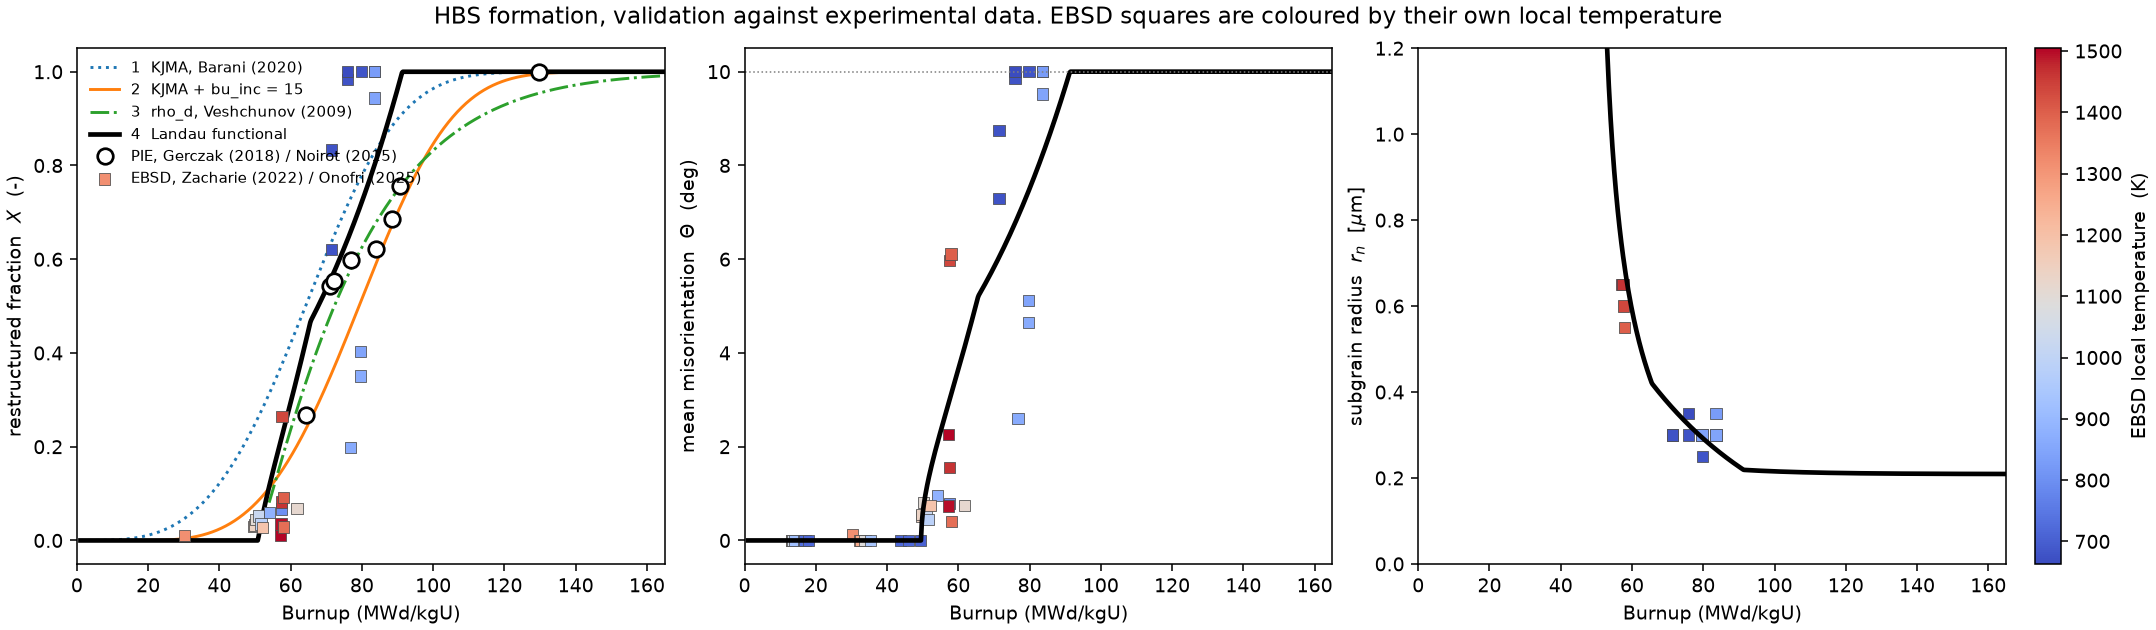
\includegraphics[width=1\textwidth]{validation.png}
  \end{center}
  \footnotesize
\end{frame}

\begin{frame}{Against the three models SCIANTIX already had}
  Burnup [MWd/kgU] at which $\alpha_r$ first reaches:

  \begin{center}
  \small
  \begin{tabular}{lrrrr}
    \toprule
    threshold & 1 KJMA & 2 KJMA$+bu_{\text{inc}}$ & 3 $\rho_d$ & \textbf{4 Landau} \\
    \midrule
    1\,\%  & 19.5  & 34.5  & 51.2  & \textbf{51.1} \\
    10\,\% & 37.8  & 52.8  & 54.8  & \textbf{53.5} \\
    50\,\% & 64.2  & 79.3  & 72.3  & \textbf{67.7} \\
    90\,\% & 90.1  & 105.2 & 112.3 & \textbf{87.7} \\
    99\,\% & 109.7 & 124.6 & 161.7 & \textbf{91.1} \\
    \bottomrule
  \end{tabular}
  \end{center}

  \begin{itemize}
    \item At the onset, option 4 lands \good{within 0.1 MWd/kgU of option 3}.
    \item They part at the top: the lever rule \alert{saturates} when $\Theta$ hits the
      $10^\circ$ cap, whereas KJMA approaches 1 asymptotically. Option 4 is done by
      91 MWd/kgU, option 3 not before 162.
    \item Option 4 spans the transition in \textbf{40 MWd/kgU} against 90 for option 1.
  \end{itemize}
\end{frame}

% =====================================================================
\section{Model applied to SCIANTIX}
% =====================================================================

\begin{frame}{Does the new formation model disturb the porosity model?}
  \begin{columns}[T]
    \begin{column}{0.7\textwidth}
      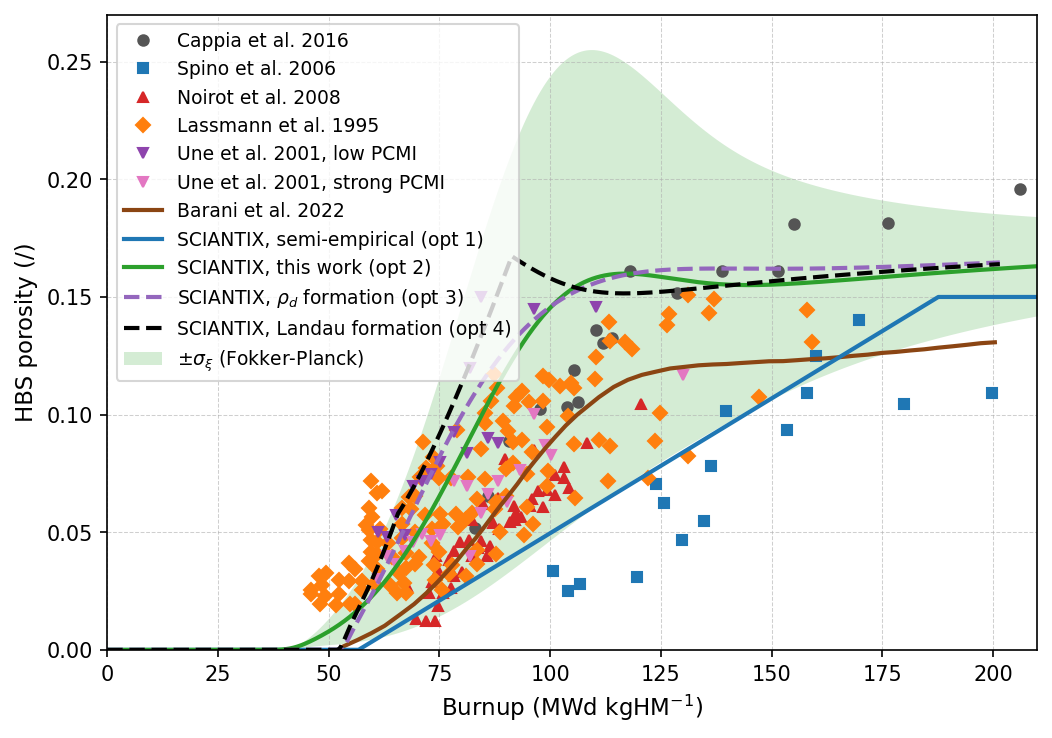
\includegraphics[width=\textwidth]{plot_porosity_landau.png}
    \end{column}
    \begin{column}{0.25\textwidth}
      \small
      \vspace{0.6em}
      Largest deviation \bad{$+0.044$ absolute at 91.3\,MWd/kgHM} ($+36\,\%$), exactly
      the saturation burnup.
      \vspace{0.4em}
      \footnotesize
      Held against option 2 in \texttt{test\_UO2HBS}; all four options end within
      \good{0.17\,\%} of the same porosity.
    \end{column}
  \end{columns}
\end{frame}

% =====================================================================
\section{Outlook: from a local functional to a phase field}
% =====================================================================

\begin{frame}{What a local functional cannot give -> phase-field models}
  \textbf{Problems of the Landau-like local functional}
  \small
  \begin{itemize}
    \item \textbf{no spatial quantities};
    \item \textbf{no kinetics}: equilibrium is instantaneous.
  \end{itemize}

  \scriptsize
  \begin{tabular}{p{0.17\textwidth}p{0.44\textwidth}p{0.25\textwidth}}
    \toprule
    family & property & application/ref \\
    \midrule
    \textbf{KWC} 
     & two fields $(\phi,\theta)$, allows subgrain rotation; singular diffusion equations
     & Nucleation via subgrain coalescence, Muramatsu (2014) \\
    \textbf{MPF} 
     & One order parameter per grain; stable time increments; rotation ignored
     & Subgrain growth, Khajezade \emph{et al.} (2024) \\
    \textbf{HMP}
     & Removes nonphysical linear gradient term; handles inclination-dependent GB energy 
     & Coupled Cosserat crystal plasticity, Tandogan \emph{et al.} (2024), Ghiglione \emph{et al.} (2024) \\
    \textbf{PFC} 
     & Atomic-resolution density field; diffusive timescales 
     & Interface morphology development during solidification, Nittala (2025) \\
    \bottomrule
  \end{tabular}

  \vspace{0.2em}
  \footnotesize
  Nucleation is usually \alert{seeded ad hoc} at a critical density or stress;
      spontaneous nucleation from lattice-curvature gradients is obtained when coupling KWC
      with Cosserat crystal plasticity (Ghiglione, 2024).

\end{frame}

\begin{frame}{Muramatsu \emph{et al.}~(2014): a KWC phase field for recrystallization}
  \footnotesize
  \begin{columns}[T]
    \begin{column}{0.52\textwidth}
      \textbf{The functional}\footnotemark[7] --- two fields, $\phi$ and $\theta$:
      \[ \mathcal{F} = \int_V \Big[\, f(\phi) + \tfrac{\alpha^2}{2}|\nabla\phi|^2
         + s\,g(\phi)\,|\nabla\theta| + \tfrac{\epsilon^2}{2}\,h(\phi)\,|\nabla\theta|^2
         \Big]\,\mathrm{d}V \]
      with $g(\phi) = h(\phi) = \phi^2$, relaxed by
      $\dot\phi = -M_\phi\,\delta\mathcal{F}/\delta\phi$ and
      $\dot\theta = -M_\theta\,\delta\mathcal{F}/\delta\theta$.

      $\phi = 1$ inside a subgrain; $\theta$ is the
      \textbf{lattice orientation}. 
      
      The \emph{singular} $|\nabla\theta|$ term gives a boundary
      an energy growing with misorientation.
    \end{column}
    \begin{column}{0.44\textwidth}
      \textbf{The local part} (Eq.~7, $f_m = 0$):
      \[ f(\phi;E_s) = a_{ub}\big(1-p(\phi)\big)E_s + a_{wg}W_b\,q(\phi) \]
      \[ q(\phi) = \phi^2(1-\phi)^2 \]
      \[ p(\phi) = \phi^3(10-15\phi+6\phi^2) \]

        \scriptsize
      \begin{itemize}
        \item $q$: the \textbf{double well}, original matrix against new grains; its height $a_{wg}W_b$
          sets the boundary energy;
        \item $p$: is a sigmoid-like function where $p'(0)=p'(1)=0$m therefore it \emph{tilts} the well without
          moving its two minima;
        \item $E_s$: the \textbf{stored dislocation energy}, the only driving force, supplied
          from outside the model.
      \end{itemize}
    \end{column}
  \end{columns}
  \textbf{How the paper nucleates}: a subgrain group enclosed by high-angle ($>10^\circ$)
  boundaries is \emph{selected} as a nucleus candidate and grows after an \emph{incubation
  period} --- the criterion is \alert{imposed}, not produced by the free energy.
\end{frame}

\begin{frame}{The prototype: the Landau model supplies the driving force}
      \scriptsize
      Keep $q(\phi)$ and $p(\phi)$ exactly as above, and replace the externally supplied $E_s$
      by what the Landau model:
      \[ f_{\text{Mur}}(\phi;E_s) = a_{ub}\big(1-p(\phi)\big)E_s + a_{wg}W_b\,q(\phi) \]
      \[ f_{\text{new}}(\phi;bu,T) = C_0\big(1-p(\phi)\,\eta\big) + a_{wg}W_b\,q(\phi) \]
      Both $C_0$ and $\eta$ come from the same \texttt{hbs\_state($bu$,$T$)} that produces
      $\Theta$, $r_n$ and $X$.

      \begin{center}
      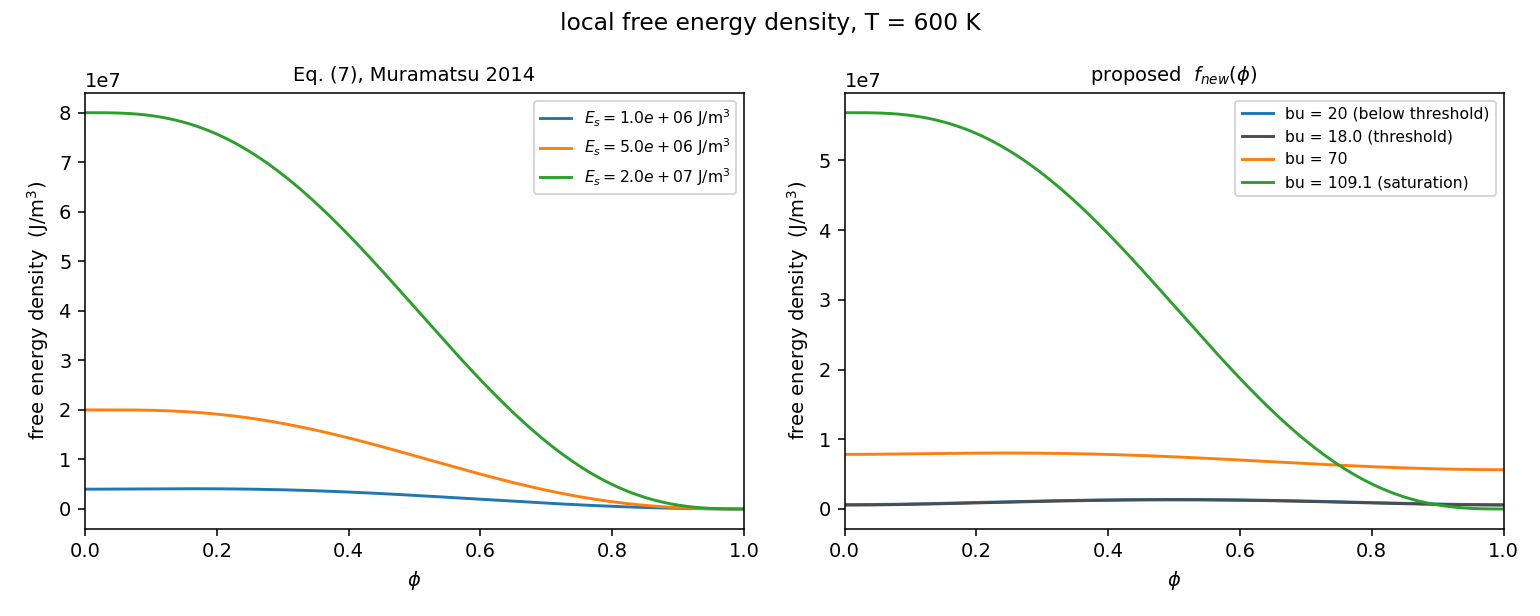
\includegraphics[width=0.7\textwidth]{phasefield_free_energy.png}

      \scriptsize
      Left: Eq.~(7) at three stored energies. Right: $f_{\text{new}}$ below, at, and above the
      threshold.
      \end{center}
\end{frame}

\begin{frame}[standout]
  Summary
\end{frame}


\appendix

% =====================================================================
\begin{frame}[allowframebreaks]{References}
  \scriptsize
  \begin{thebibliography}{99}
    \setbeamertemplate{bibliography item}[text]

    \bibitem{landau1937} L.D.\ Landau,
      \emph{On the theory of phase transitions}, Zh.\ Eksp.\ Teor.\ Fiz.\ \textbf{7} (1937) 19;
      L.D.\ Landau, E.M.\ Lifshitz, \emph{Statistical Physics}, Part 1, 3rd ed., \S143.

    \bibitem{kolmogorov1937} A.N.\ Kolmogorov,
      Izv.\ Akad.\ Nauk SSSR, Ser.\ Mat.\ \textbf{1} (1937) 355--359.

    \bibitem{johnsonmehl1939} W.A.\ Johnson, R.F.\ Mehl,
      Trans.\ AIME \textbf{135} (1939) 416--442.

    \bibitem{avrami1939} M.\ Avrami,
      \emph{J.\ Chem.\ Phys.} \textbf{7} (1939) 1103--1112; \textbf{8} (1940) 212--224;
      \textbf{9} (1941) 177--184.

    \bibitem{christian2002} J.W.\ Christian,
      \emph{The Theory of Transformations in Metals and Alloys}, Part I, 3rd ed.,
      Pergamon (2002), ch.\ 12, \emph{Formal Theory of Transformation Kinetics}.

    \bibitem{humphreys1997} F.J.\ Humphreys,
      \emph{A unified theory of recovery, recrystallization and grain growth, based on the
      stability and growth of cellular microstructures --- I. The basic model},
      \emph{Acta Mater.} \textbf{45} (1997) 4231--4240.

    \bibitem{humphreys2017} F.J.\ Humphreys, G.S.\ Rohrer, A.D.\ Rollett,
      \emph{Recrystallization and Related Annealing Phenomena}, 3rd ed., Elsevier (2017),
      ch.\ 6 (recovery) and ch.\ 10 (growth and stability of cellular microstructures).

    \bibitem{gourdet2003} S.\ Gourdet, F.\ Montheillet,
      \emph{A model of continuous dynamic recrystallization},
      \emph{Acta Mater.} \textbf{51} (2003) 2685--2699.
      \hfill{\itshape $n$, and the sweeping term}

    \bibitem{readshockley1950} W.T.\ Read, W.\ Shockley,
      \emph{Dislocation models of crystal grain boundaries},
      \emph{Phys.\ Rev.} \textbf{78} (1950) 275--289.
      \hfill{\itshape $\theta = b/d$, and the wall energy}

    \bibitem{nye1953} J.F.\ Nye,
      \emph{Some geometrical relations in dislocated crystals},
      \emph{Acta Metall.} \textbf{1} (1953) 153--162.

    \bibitem{rohrer2011} G.S.\ Rohrer,
      \emph{Grain boundary energy anisotropy: a review},
      \emph{J.\ Mater.\ Sci.} \textbf{46} (2011) 5881--5895.

    \bibitem{resthofman2000} J.\ Rest, G.L.\ Hofman,
      \emph{An alternative explanation for evidence that xenon depletion, pore formation and
      grain subdivision begin at different local burnups},
      \emph{J.\ Nucl.\ Mater.} \textbf{277} (2000) 231--238.
      \hfill{\itshape the analogue of $\beta$}

    \bibitem{kwc2000} R.\ Kobayashi, J.A.\ Warren, W.C.\ Carter,
      \emph{A continuum model of grain boundaries},
      \emph{Physica D} \textbf{140} (2000) 141--150.
      \hfill{\itshape the $(\phi,\theta)$ functional}

    \bibitem{muramatsu2014} M.\ Muramatsu, Y.\ Aoyagi, Y.\ Tadano, K.\ Shizawa,
      \emph{Phase-field simulation of static recrystallization considering nucleation from
      subgrains and nucleus growth with incubation period},
      \emph{Comput.\ Mater.\ Sci.} \textbf{87} (2014) 112--122.

    \bibitem{chen2002} L.-Q.\ Chen,
      \emph{Phase-field models for microstructure evolution},
      \emph{Annu.\ Rev.\ Mater.\ Res.} \textbf{32} (2002) 113--140.
      \hfill{\itshape the general framework}

    \bibitem{takaki2007} T.\ Takaki, A.\ Yamanaka, Y.\ Tomita,
      \emph{Phase-field modeling and simulation of nucleation and growth of recrystallized
      grains}, \emph{Mater.\ Sci.\ Forum} \textbf{558--559} (2007) 1195--1200.
      \hfill{\itshape KWC, subgrain rotation}

    \bibitem{muramatsu2008} M.\ Muramatsu, Y.\ Tadano, K.\ Shizawa,
      \emph{A phase-field simulation of nucleation from subgrain and grain growth in static
      recrystallization}, \emph{Mater.\ Sci.\ Forum} \textbf{584--586} (2008) 1045--1050.
      \hfill{\itshape nucleation by coalescence}

    \bibitem{khajezade2024} A.\ Khajezade, W.\ Poole, M.\ Greenwood, M.\ Militzer,
      \emph{Large-scale multi-phase-field simulation of 2D subgrain growth},
      \emph{Metals} \textbf{14} (2024) 584.
      \hfill{\itshape MPF, Read--Shockley}

    \bibitem{tandogan2024} I.T.\ Tandogan, M.\ Budnitzki, S.\ Sandfeld,
      \emph{A multi-physics model for the evolution of grain microstructure},
      \emph{Int.\ J.\ Plast.} \textbf{180} (2024) 104201.
      \hfill{\itshape HMP orientation field}

    \bibitem{tandogan2025} I.T.\ Tandogan, M.\ Budnitzki, S.\ Sandfeld,
      \emph{A multi-physics model for dislocation driven spontaneous grain nucleation and
      microstructure evolution in polycrystals},
      \emph{J.\ Mech.\ Phys.\ Solids} (2025) 106325.

    \bibitem{ghiglione2024} F.\ Ghiglione, A.\ Ask, K.\ Ammar, B.\ Appolaire, S.\ Forest,
      \emph{Cosserat-phase-field modeling of grain nucleation in plastically deformed single
      crystals}, \emph{J.\ Mech.\ Phys.\ Solids} \textbf{188} (2024) 105628.
      \hfill{\itshape spontaneous nucleation}

    \bibitem{kong2018} L.\ Kong \emph{et al.},
      \emph{A study of strain-driven nucleation and extension of deformed grain: phase field
      crystal and continuum modeling}, \emph{Materials} \textbf{11} (2018) 1805.

    \bibitem{nittala2025} S.\ Nittala \emph{et al.},
      \emph{Interface morphology and dislocation-mediated processes during rapid solidification
      of thin films}, \emph{Acta Mater.} (2025) 121581.
      \hfill{\itshape PFC subgrain boundaries}

    \bibitem{barani2020} T.\ Barani \emph{et al.},
      \emph{Modeling high burnup structure in oxide fuels\dots\ Part I: HBS formation},
      \emph{J.\ Nucl.\ Mater.} \textbf{539} (2020) 152296.
      \hfill{\itshape option 1}

    \bibitem{barani2022} T.\ Barani \emph{et al.},
      \emph{\dots\ Part II: Porosity evolution},
      \emph{J.\ Nucl.\ Mater.} \textbf{563} (2022) 153627.
      \hfill{\itshape porosity options 2--3}

    \bibitem{biswas2025} S.\ Biswas, L.K.\ Aagesen,
      \emph{Comput.\ Mater.\ Sci.} \textbf{258} (2025) 114052, Eq.\ 45.
      \hfill{\itshape option 2, $bu_{\text{inc}}$}

    \bibitem{veshchunov2009} M.S.\ Veshchunov, V.E.\ Shestak,
      \emph{Model for evolution of crystal defects in UO$_2$ under irradiation up to high
      burn-ups}, \emph{J.\ Nucl.\ Mater.} \textbf{384} (2009) 12--18.
      \hfill{\itshape option 3, $\rho_d(bu,T)$}

    \bibitem{khvostov2005} G.\ Khvostov \emph{et al.},
      \emph{Approaches to modeling of high burn-up structure\dots\ in the START-3 code},
      WRFPM-2005, Kyoto.

    \bibitem{nogita1994} K.\ Nogita, K.\ Une,
      \emph{Radiation-induced microstructural change in high burnup UO$_2$ fuel pellets},
      \emph{Nucl.\ Instrum.\ Methods B} \textbf{91} (1994) 301--306.
      \hfill{\itshape Eq.~(1), $\rho_{\text{tot}}(bu)$}

    \bibitem{nogita1995} K.\ Nogita, K.\ Une,
      \emph{Irradiation-induced recrystallization in high burnup UO$_2$ fuel},
      \emph{J.\ Nucl.\ Mater.} \textbf{226} (1995) 302--310.

    \bibitem{matzke1997} Hj.\ Matzke, M.\ Kinoshita,
      \emph{Polygonization and high burnup structure in nuclear fuels},
      \emph{J.\ Nucl.\ Mater.} \textbf{247} (1997) 108--115.

    \bibitem{spino2006} J.\ Spino \emph{et al.},
      \emph{J.\ Nucl.\ Mater.} \textbf{354} (2006) 66--84.
      \hfill{\itshape porosity option 1, and the swelling data}

    \bibitem{zacharie2022} I.\ Zacharie-Aubrun \emph{et al.},
      \emph{Restructuring in high burn-up UO$_2$ fuels: experimental characterization by
      electron backscattered diffraction},
      \emph{J.\ Appl.\ Phys.} \textbf{132} (2022) 195903.
      \hfill{\itshape 28 of the 42 EBSD points}

    \bibitem{onofri2025} C.\ Onofri \emph{et al.},
      \emph{Experimental characterizations by EBSD and TEM of sub-grain boundaries and
      dislocations in low irradiated UO$_2$ fuels},
      \emph{J.\ Nucl.\ Mater.} \textbf{615} (2025) 155981.
      \hfill{\itshape the other 14}

    \bibitem{nea2024} NEA,
      \emph{Recommendations on nuclear fuel properties}, NEA/NSC/R(2024)1 (2025), p.\ 124.
      \hfill{\itshape Eq.~(2), $G$ and $\nu$}

    \bibitem{pizzocri2020} D.\ Pizzocri \emph{et al.},
      \emph{SCIANTIX: a new open source multi-scale code for fission gas behaviour modelling},
      \emph{J.\ Nucl.\ Mater.} \textbf{532} (2020) 152042.

    \bibitem{zullo2023} G.\ Zullo \emph{et al.},
      \emph{The SCIANTIX code for fission gas behaviour: status, upgrades, separate-effect
      validation and future developments},
      \emph{J.\ Nucl.\ Mater.} \textbf{587} (2023) 154744.

  \end{thebibliography}
\end{frame}


\begin{frame}{Backup --- the equations}
  \scriptsize
  \begin{align*}
    \text{(1)}\;\; & \rho_{\text{tot}}(bu) = 10^{2.2\times10^{-2} bu + 13.8} \\
    \text{(2)}\;\; & G(T,P,x,q),\ \nu(T,P,x,q) \quad \text{NEA/NSC/R(2024)1 p.\ 124};\quad f(\nu) = \tfrac{1-\nu/2}{1-\nu} \\
    \text{(3)}\;\; & \rho^{\max}_{\text{LAGB}} = \Big(\tfrac{3n\theta_{\max}}{\beta b}\Big)^2,\quad
                     (S/V)_{\max} = \tfrac{9n\theta_{\max}}{\beta^2 b},\quad
                     \tfrac{\Delta R}{R}\Big|_{\max} = \tfrac{k\,\rho^{\max}_{\text{LAGB}}}{\rho_{\text{tot}}} \\
    \text{(4)}\;\; & A_1 = \tfrac{f(\nu)}{4\pi}\ln\tfrac{\rho_c^{-1/2}}{b},\qquad
                     A_2 = \tfrac{f(\nu)}{4\pi}\ln\tfrac{\rho_{\text{tot}}^{-1/2}}{b} \\
    \text{(5,6)}\; & F = \rho_{\text{free}}A_1Gb^2 + \rho_{\text{ord}}A_2Gb^2 = C_0 + C_2\eta^2 + C_4\eta^4 \\
    \text{(7,7b)}\;& \eta_{\text{eq}} = \min\!\big(\sqrt{-C_2/2C_4},\ \eta_{\text{bal}}\big),\quad
                     \eta_{\text{bal}} = \sqrt{\min(\rho_{\text{tot}}/\rho^{\max}_{\text{LAGB}},1)} \\
    \text{(8)}\;\; & \Theta = \min(\eta_{\text{eq}}\theta_{\max}\cdot\tfrac{180}{\pi},\ \theta_{\text{HAGB}}) \\
    \text{(9)}\;\; & r_n = \min\!\big(\tfrac{1.5}{(S/V)}(1+\tfrac{\Delta R}{R}),\ R_{\text{grain}}\big) \\
    \text{(10)}\;\;& X = \mathrm{clip}\big(\tfrac{\Theta-\theta_u}{\theta_{\text{HAGB}}-\theta_u},\,0,\,1-10^{-9}\big)
  \end{align*}
\end{frame}

\begin{frame}{Backup --- regimes and parameters}
  \begin{columns}[T]
    \begin{column}{0.5\textwidth}
      \textbf{Regimes} ($T$-, $P$-, $x$-independent)
      \small
      \begin{tabular}{lr}
        \toprule
        condition & $bu$ [GWd/tU] \\
        \midrule
        $C_2 = 0$, $\Theta$ leaves 0     & 49.56 \\
        $\Theta = \theta_u$, $X$ leaves 0 & 50.81 \\
        $\Theta = \theta_{\text{HAGB}}$   & 91.32 \\
        \bottomrule
      \end{tabular}

      \vspace{0.8em}
      The balance bound sets $\eta$ over roughly \textbf{65.6--91.3 GWd/tU}, and at
      11 of the 41 EBSD points.
    \end{column}
    \begin{column}{0.5\textwidth}
      \textbf{Fixed constants}
      \small
      \begin{tabular}{lr}
        \toprule
        $b$ & 3.889e-10 m \\
        $\theta_{\max}$ & $= \theta_{\text{HAGB}}$ \\
        $\theta_{\text{HAGB}}$ & $10^\circ$ \\
        $\theta_u$ & $1.00^\circ$ \\
        $n$ & 2 \\
        \bottomrule
      \end{tabular}

      \vspace{0.6em}
      \footnotesize
      $\theta_u$ is the lower end member of the mixture Eq.~(10) inverts, and it is set by
      the \textbf{measurement convention}, not fitted: the EBSD data reports a restructured
      fraction \emph{at} $1^\circ$ ($f_1$) and one \emph{at} $10^\circ$ ($f_{10}$), so
      $1^\circ$ is the edge below which a boundary is not counted at all. A map whose whole
      resolved population sits there carries no restructuring --- which is $X = 0$.
      It fixes only \emph{where} $X$ leaves zero: $\Theta$ and $r_n$ do not depend on it.
    \end{column}
  \end{columns}
\end{frame}

\begin{frame}{Backup --- the model on its own, $T = 600$\,K, $P = 0.05$}
  \begin{center}
    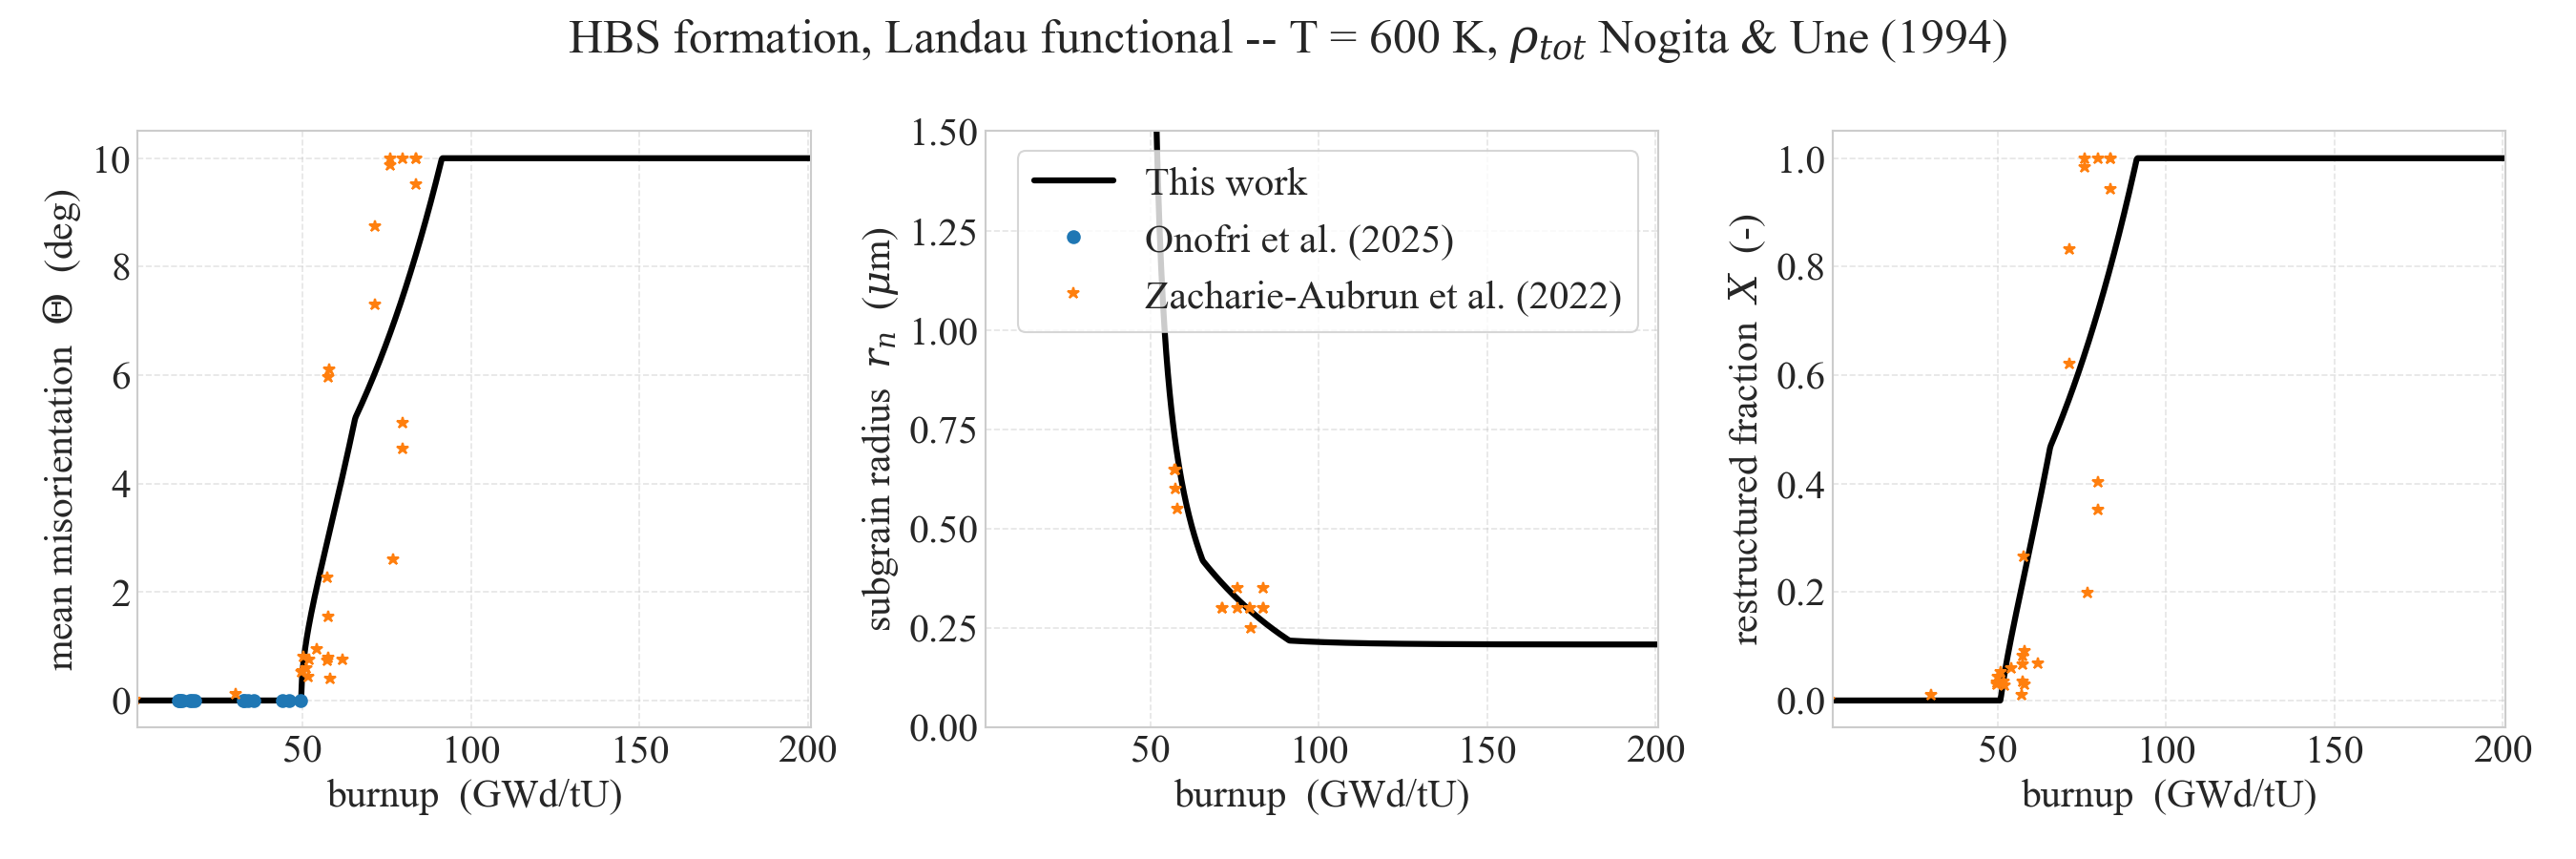
\includegraphics[width=0.86\textwidth]{hbs_formation_landau.png}
  \end{center}
  \footnotesize
  \texttt{python3 hbs\_formation\_landau.py -{}-plot}
\end{frame}

\begin{frame}{Backup --- the four regression cases, as they ship}
  \begin{columns}[T]
    \begin{column}{0.62\textwidth}
      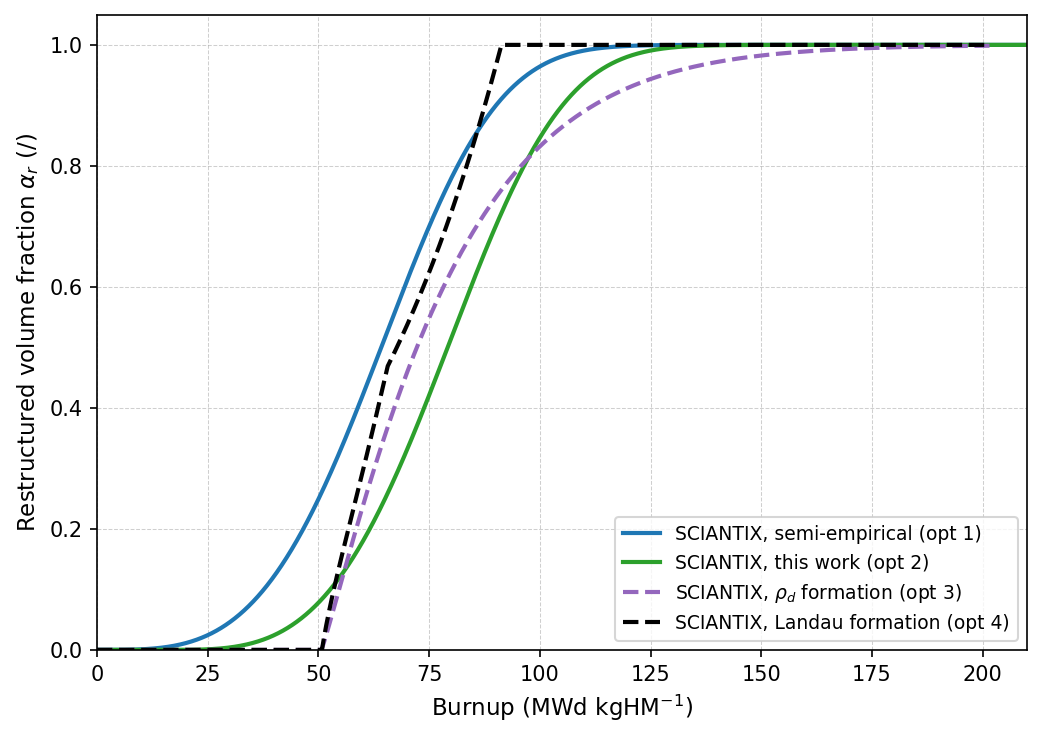
\includegraphics[width=\textwidth]{plot_alpha_r_landau.png}
    \end{column}
    \begin{column}{0.35\textwidth}
      \footnotesize
      \alert{Not} the controlled comparison of the previous figure: each case pairs its
      formation option with the porosity model it was built around (1, 2, 3, 3), so part
      of the spread is the porosity model.

      \vspace{0.5em}
      This is what a user of each regression case actually gets;
      \texttt{formation\_options.png} is what isolates the formation model.
    \end{column}
  \end{columns}
\end{frame}

\begin{frame}{Backup --- the four formation options in a full run}
  \begin{center}
    
\includegraphics[width=0.95\textwidth]{formation_options.png}
  \end{center}
\end{frame}

\end{document}
